\documentclass[11pt]{article}
\usepackage{graphicx} 
\usepackage[margin=0.5in]{geometry}

\title{Notes on Intensive Embedding for 1-Spin Model}
\author{Katherine Quinn}

\begin{document}

\maketitle

In the 1-Spin model, we have a certain probability of finding the spin up, $\rho$, and a certain probability of finding the spin down ($1-\rho$), where $\rho$ ranges from 0 to 1. This forms likelihood function, $\mathcal{L}_\rho = (\rho,1-\rho)$. When looking at the prediction space for this model, if we look at $\mathcal{L}$ we would get a line. If instead we look at $(\sqrt{\rho},\sqrt{1-\rho})$ we get a quarter of a hemi-sphere. If we reparametrise, so that $\sqrt{\rho}=\sin{\theta}$ and consider our \textit{intensive embedding}, given by:
\begin{eqnarray}
d^2(\theta_1,\theta_2) = -2\log\left(\sin(\theta_1)\sin(\theta_2)+\cos(\theta_1)\cos(\theta_2) \right) = -2\log\cos(\theta_1-\theta_2)
\end{eqnarray}

This produces the following model manifold:

\begin{center}
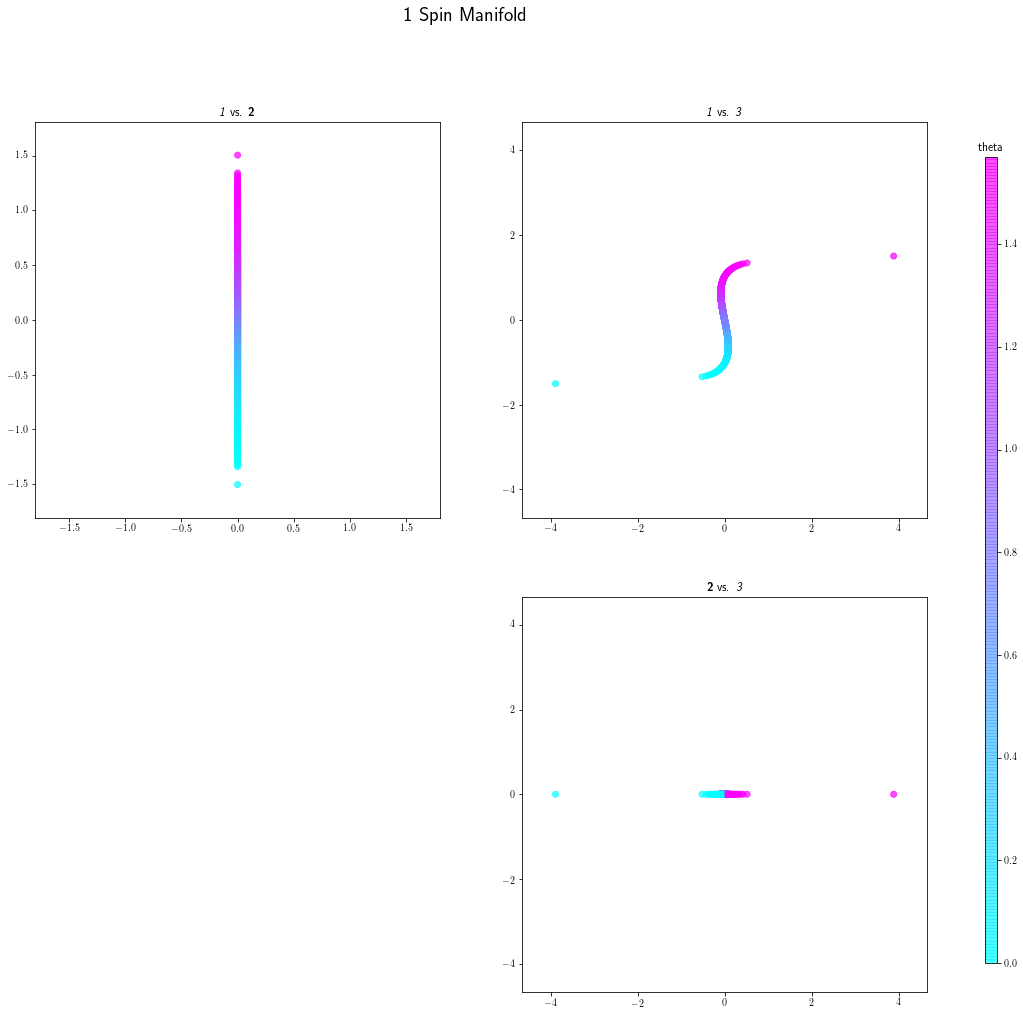
\includegraphics[width=6in]{./manifold.png}
\end{center}

Where the real/positive square distances are shown in italics (1 and 3) and the imaginary/negative squared distances are indicated by bolding (3). Points are colored by parameter angle $\theta$.

Distance between points, in parameter space for some small perturbation in parameters $\delta\theta$, is given by the metric $g_\mu\nu$:
\begin{eqnarray}
d^2(\theta,\theta+\delta\theta) = g_{\mu\nu}\delta\theta^\mu\delta\theta^\nu
\end{eqnarray}
Where the metric is parameter dependent. In our embedding space, the metric is imply diagonal with $\pm 1$. If we look at the distance between points in the embedding space, we get the following plot which compares the contribution from the real and imaginary components:

\begin{center}
\includegraphics[width=6in]{./distances.png}
\end{center}

Where the red line shows the contribution from the real component, and the green shows it from the imaginary component. The total distance is given by the black line, and is always real. In parameter space, $g_\mu\nu$ is given by the Fisher Information Metric, which for our case is:
\begin{eqnarray}
g_{\mu\nu} &=& \sum_x \partial_\mu\log\mathcal{L}(x|\theta)\partial_\nu\log\mathcal{L}(x|\theta)\mathcal{L}(x|\theta)\nonumber\\
g_{\theta\theta} &=& \left(\partial_\theta\log\cos^2\theta\right)^2\cos^2\theta + \left(\partial_\theta\log\sin^2\theta\right)^2\sin^2\theta \nonumber\\
&=& 4
\end{eqnarray}

The FIM distance and the ``Euclidean" distance are related: the ``Euclidean" distance is calculated by considering a limiting case of the Hellinger distance, which does contain as a metric in parameter space the FIM.

We can treat our distance function as an infinite matrix, acting on continuous variables $\phi$ and $\theta$: $\log\cos(\phi-\theta)$. We can find the Eigenvalues and Eigenfunctions of this, by solving the following:
\begin{eqnarray}
\int_0^{\pi/2}\texttt{d}\theta\log\cos(\phi - \theta)v_\alpha (\theta) = \lambda_\alpha v_\alpha(\phi)
\end{eqnarray}
where $v_\alpha(\theta)$ are the Eigenfunctions with corresponding Eigenvalues $\lambda_\alpha$. Solving this numerically with python, we get the following:

\begin{center}
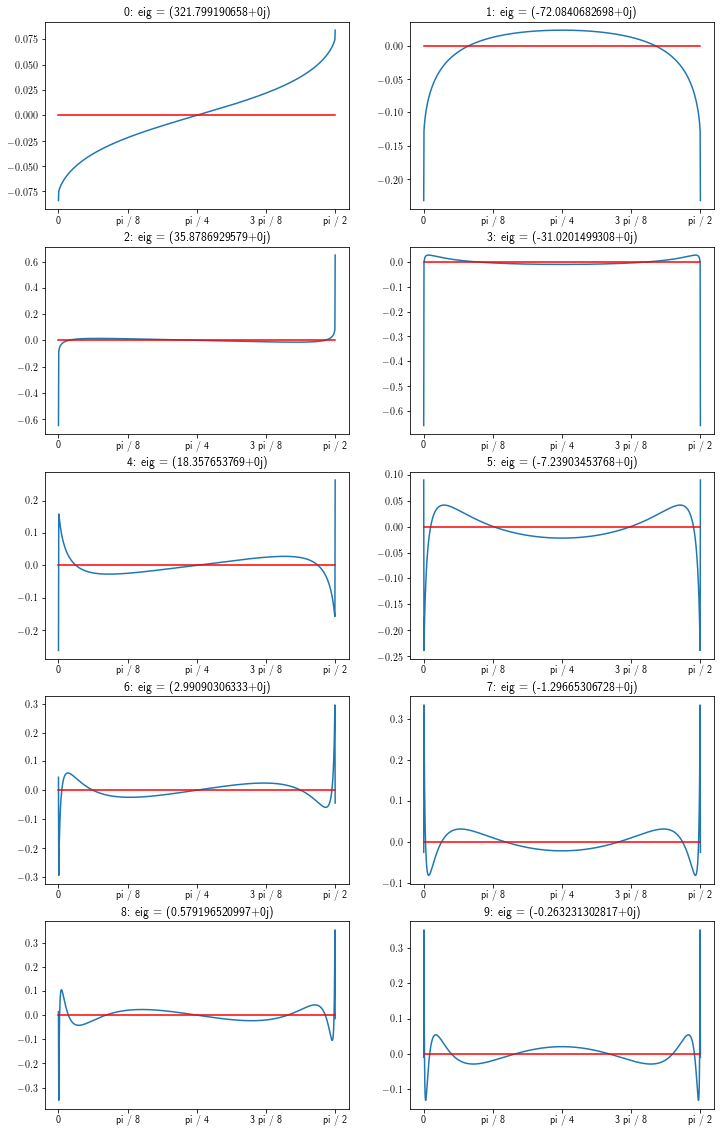
\includegraphics[width=6in]{./eigFunctsVals.png}
\end{center}

Where we can begin to see certain patterns, such as how odd functions have positive eigenvalues and even ones have negative ones.

\end{document}